\resizebox{0.5\textwidth}{!}{%
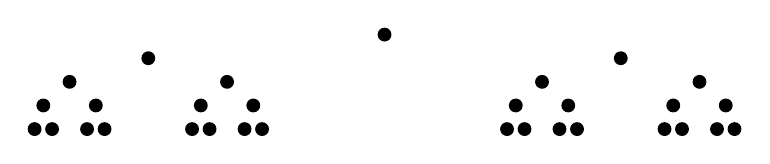
\begin{tikzpicture}[scale=1]

% Parametry
\def\ysep{0.3}
\def\rad{2.5pt}

% ---------- Krok 0: srodek odcinka [0,1] ----------
\fill[black] (4.5, 0) circle (\rad);
% \node[left] at (-0.2, 0) {$C_0$};

% ---------- Krok 1: srodki 2 odcinkow ----------
\fill[black] (1.5, -\ysep) circle (\rad);
\fill[black] (7.5, -\ysep) circle (\rad);
% \node[left] at (-0.2, -\ysep) {$C_1$};

% ---------- Krok 2: srodki 4 odcinkow ----------
\fill[black] (0.5, -2*\ysep) circle (\rad);
\fill[black] (2.5, -2*\ysep) circle (\rad);
\fill[black] (6.5, -2*\ysep) circle (\rad);
\fill[black] (8.5, -2*\ysep) circle (\rad);
% \node[left] at (-0.2, -2*\ysep) {$C_2$};

% ---------- Krok 3: srodki 8 odcinkow ----------
\fill[black] (0.1667, -3*\ysep) circle (\rad);
\fill[black] (0.8333, -3*\ysep) circle (\rad);
\fill[black] (2.1667, -3*\ysep) circle (\rad);
\fill[black] (2.8333, -3*\ysep) circle (\rad);
\fill[black] (6.1667, -3*\ysep) circle (\rad);
\fill[black] (6.8333, -3*\ysep) circle (\rad);
\fill[black] (8.1667, -3*\ysep) circle (\rad);
\fill[black] (8.8333, -3*\ysep) circle (\rad);
% \node[left] at (-0.2, -3*\ysep) {$C_3$};

% ---------- Krok 4: srodki 16 odcinkow ----------
% Srodki odcinkow dlugosci 1/81, w jednostkach skali 9:
% odcinek dlugosci 9/16, srodek w (m+0.5)*9/16 dla m=0..15
% ale z zachowaniem struktury Cantora (pomijamy usuniete przedzialy)
\fill[black] (0.0556, -4*\ysep) circle (\rad);
\fill[black] (0.2778, -4*\ysep) circle (\rad);
\fill[black] (0.7222, -4*\ysep) circle (\rad);
\fill[black] (0.9444, -4*\ysep) circle (\rad);
\fill[black] (2.0556, -4*\ysep) circle (\rad);
\fill[black] (2.2778, -4*\ysep) circle (\rad);
\fill[black] (2.7222, -4*\ysep) circle (\rad);
\fill[black] (2.9444, -4*\ysep) circle (\rad);
\fill[black] (6.0556, -4*\ysep) circle (\rad);
\fill[black] (6.2778, -4*\ysep) circle (\rad);
\fill[black] (6.7222, -4*\ysep) circle (\rad);
\fill[black] (6.9444, -4*\ysep) circle (\rad);
\fill[black] (8.0556, -4*\ysep) circle (\rad);
\fill[black] (8.2778, -4*\ysep) circle (\rad);
\fill[black] (8.7222, -4*\ysep) circle (\rad);
\fill[black] (8.9444, -4*\ysep) circle (\rad);
% \node[left] at (-0.2, -4*\ysep) {$C_4$};

% % Opcjonalnie: kropki koncowe (granica)
% \node[below] at (4.5, -4*\ysep-0.5) {$\vdots$};
% \node[below] at (4.5, -4*\ysep-1.0) {granica: zbiór Cantora $C$};

\end{tikzpicture}

}